\chapter{The Transition to Planet Formation}
\label{ch:planets}

\marginnote{
\textbf{Suggested background reading:}
\begin{itemize}
\item \href{http://adsabs.harvard.edu/abs/2014prpl.conf..547J}{Johansen, A., et al. 2014, in "Protostars and Planets VI", ed.~H.~Beuther et al., pp.~547-570} \nocite{johansen14a}
\end{itemize}
\textbf{Suggested literature:}
\begin{itemize}
\item \href{http://adsabs.harvard.edu/abs/2010ApJ...722.1437B}{Bai, X.-N., \& Stone, J.~M. 2010, ApJ, 722, 1437} \nocite{bai10a}
\end{itemize}
}

In this final chapter, we will finish our discussion of the transition from star formation to planet formation. We have already seen in chapter \ref{ch:late_disk} that the interstellar dust grains that are captured in a star's disk will begin to collide with one another and grow, and that they will reach macroscopic size on time scales shorter than the observed disk lifetime. We now seek to sharpen our understanding of how these solids will evolve. We will continue to make use of fiducial numbers from the minimum mass Solar nebula (MMSN) that we introduced in chapter \ref{ch:late_disk}.

\section{Dynamics of Solid Particles in a Disk}

\subsection{Forces on Solids}

We begin our discussion by attempting to determine the dynamics of solid particles orbiting in a protoplanetary disk. Consider such a particle. Because the mass of the disk is very small compared that of the star, we can neglect the gravitational force it exerts in the radial direction, and thus the radial gravitational acceleration felt by the particle is simply $g_\varpi = G M/\varpi^2$, where $M$ is the star's mass and $\varpi$ is the distance from the star. 

In the vertical direction we have the gravitational pull of both the star and the disk itself, and we have to think a bit more. However, one can show fairly easily that, for material distributed with the thermal scale height of the disk, the star's vertical gravity must dominate as well. The star's vertical gravitational force is 
\begin{equation}
g_{z,*} = \frac{z}{\varpi} g_\varpi = \Omega^2 z,
\end{equation}
where $z$ is the distance above the disk midplane and $\Omega$ is the angular velocity of a Keplerian orbit. We can approximate the disk as an infinite slab of surface density $\Sigma$; the gravitational force per unit mass exerted by such a slab is
\begin{equation}
g_{z,d} = 2\pi G \Sigma.
\end{equation}
The ratio of the stellar force to the disk force at a distance $H$ off the midplane, the typical disk height, is
\begin{equation}
\frac{g_{z,*}}{g_{z,d}} = \frac{\Omega^2 H}{2\pi G \Sigma} = \frac{c_g \Omega}{2\pi G \Sigma} = \frac{Q}{2},
\end{equation}
where in the last step we substituted in the Toomre $Q=\Omega c_g/(\pi G \Sigma)$ for a Keplerian disk.

Thus the vertical gravity of the disk is negligible as long as it is Toomre stable, $Q\gg 1$. For our MMSN,
\begin{equation}
\label{eq:QMMSN}
Q=55 \varpi_0^{-1/4},
\end{equation}
so unless we are {\it very} far out, stellar gravity completely dominates. As a caveat, it is worth noting that we implicitly assumed that the scale height $H$ applies to both the gas and the dust, even though we calculated it only for the gas. In fact, the motion of the dust is more complex, and, as we will see shortly, the assumption that the dust scale height is the same as that of the gas is not a good one. Nonetheless, neglecting the self-gravity of the disk is a reasonable approximation until significant gas-dust separation has occurred.

The other force on the solids that we have to consider is drag. Aerodynamic drag is a complicated topic, but we can get an estimate of the drag force for a small, slowly moving particle that is good to order unity fairly easily. Consider a spherical particle of size $s$ moving through a gas of density $\rho$ and sound speed $c_g$ at a velocity $v$ relative to the mean velocity of the gas. First note that for small particles the mean free path of a gas molecule is larger than the particle size -- Problem Set 5 contains a computation of the size scale up to which this remains the case.

For such small grains it is a reasonable approximation to neglect collective behavior of the gas and view it as simply a sea of particles whose velocity distribution does not change in response to the dust grain moving through it. If the particle is moving slowly compared to the molecules, which will be the case for most grains, then the rate at which molecules strike the grain surface will be
\begin{equation}
\mbox{collision rate} \approx 4\pi s^2 \frac{\rho}{\mu m_{\rm H}} c_g,
\end{equation}
where $\mu$ is the mean mass per molecule, so $\rho/\mu m_{\rm H}$ is the number density. This formula simply asserts that the collision rate is roughly equal to the grain area times the number density of molecules times their mean speed.

If the grain were at rest the mean momentum transferred by these collisions would be zero. However, because it is moving, collisions on the forward face happen at a mean velocity of $\sim c_g+v$, and those on the backward face have a mean velocity $\sim c_g-v$. Thus, averaging over many collisions, there will be a net momentum transfer per collision of $\mu m_{\rm H} v$. The net rate of momentum transfer, the drag force, is therefore the product of this with the collision rate:
\begin{equation}
F_D = C_D s^2 \rho v c_g,
\end{equation}
where $C_D$ is a constant of order unity.

Integrating over the Boltzmann distribution and assuming that all collisions are elastic and that the reflectance is in random directions (so-called diffuse reflection), appropriate for a rough surface, gives $C_D = 4\pi/3$. With this value of $C_D$, this formula is known as the Epstein drag law. It becomes exact in the limit $s\ll \mbox{mean free path}$, $v \ll c_g$, and for pure elastic, diffuse reflection. Larger bodies experience Stokes drag, in which the dependence changes from $s^2 \rho v c_g$ to $s^2 \rho v^2$, but we will not worry about that for now. Finally, note that solid particles will not experience significant pressure forces, since they are so much more massive than the molecules that provide pressure.

\subsection{Settling}

Now let us consider what the combination of vertical gravity and drag implies. The vertical equation of motion for a particle is
\begin{equation}
\frac{d^2 z}{dt^2} = -g_z - \frac{F_D}{\frac{4}{3}\pi s^3 \rho_s} = -\Omega^2 z - \frac{\rho c_g}{\rho_s s} \frac{dz}{dt}
\end{equation}
where $\rho_s$ is the density of the solid particle. This ODE represents a damped harmonic oscillator: the gravitational term is the linear restoring force, and the drag term is the damping term. Within one gas scale height of the midplane $\rho$ is roughly constant, $\rho \approx \Sigma/H = 3\times 10^{-9} \varpi_0^{-11/4}$ g cm$^{-3}$. For constant $\rho$ the ODE can be solved analytically:
\begin{equation}
z = z_0 e^{-t/\tau},
\end{equation}
where
\begin{equation}
\tau = 2\frac{\rho_s s}{\rho c_g} \left[1 - \left(1 - \frac{4 s^2 \rho_s^2 \Omega^2}{\rho^2 c_g^2}\right)^{1/2}\right]^{-1}.
\end{equation}

If the term in the square root is negative, which is the case when $s$ is large, the damping is not strong enough to stop particles before they reach the midplane, and they instead perform a vertical oscillation of decreasing magnitude. If it is positive, they simply drift downward, approaching the midplane exponentially. The minimum time to reach the midplane occurs when the particles are critically damped, corresponding to the case where the square root term vanishes exactly. Critical damping occurs for particles of size
\begin{equation}
s_c = \frac{\rho c_g}{2 \rho_s \Omega} = 850 \varpi_0^{-3/2} \rho_{s,0}^{-1}\mbox{ cm},
\end{equation}
where $\rho_{s,0} = \rho_s/(1\mbox{ g cm}^{-3})$.

Thus all objects smaller than $\sim 10$ m boulders will slowly drift down to the midplane without oscillating. For $s\ll s_c$, we can expand the square root term in a series to obtain
\begin{equation}
\tau \approx 4 \frac{\rho_s s}{\rho c_g} \left(\frac{s}{s_c}\right)^{-2} = \frac{\rho c_g}{\rho_s \Omega^2 s} = 270 \varpi_0^{11/4} \rho_{s,0}^{-1} s_0^{-1}\mbox{ yr},
\end{equation}
where $s_0 = s/(1\mbox{ cm})$. 

Thus 1 cm grains will settle to the midplane almost immediately, while interstellar grains, those $\sim 1$ $\mu$m in size, will take several Myr to reach the midplane. Of course these very small grains will also collide with one another and grow to larger sizes, which will let them sediment more rapidly. In practice coagulation and sedimentation occur simultaneously, and each enhances the other: growth helps particle sediment faster, and sedimentation raises the density, letting them collide more often.

\subsection{Radial Drift}

We have just considered the consequences of the forces acting on solid particles in the vertical direction. Next let us consider the radial direction. The homework includes a detailed solution to this problem for small particles, so we will not go through the calculation, just the qualitative result. The basic idea is that gas in the disk is mostly supported by rotation, but it also has some pressure support. As a result, it orbits at a slightly sub-Keplerian velocity. Solid bodies, on the other hand, do not feel gas pressure, so they can only remain in orbit at constant radius if they orbit at the Keplerian velocity. The problem is that this means that they are moving faster than the gas, and thus experience a drag force.

Problem Set 5 contains a calculation showing that the difference in velocity between the Keplerian speed and the speed with which a particle orbits is
\begin{equation}
\Delta v = \frac{n c_g^2}{2 v_K} = \eta v_K
\end{equation}
where the pressure in the disk is assumed to vary with distance from the star as $P\propto \varpi^{-n}$, $c_g$ is the gas sound speed, and the dimensionless quantity $\eta = n c_g^2/2 v_K^2$, which depends only on the local properties of the disk, has been defined for future convenience. At 1 AU for our minimum mass solar nebula model, this velocity is about $70 n$ m s$^{-1}$.

Drag takes away angular momentum, in turn causing the bodies to spiral inward. We can parameterize this effect in terms of the stopping time 
\begin{equation}
t_s = \frac{mv}{F_D},
\end{equation}
where $m$ and $v$ are the body's mass and velocity, and $F_D$ is the drag force it experiences. The stopping time is simply the characteristic time scale required for drag to stop the body.

Consider a spherical solid body of size $s$. For the Epstein law, which we discussed last time, $F_D \propto s^2$, while for Stokes drag, which describes larger bodies, $F_D \propto s^2$ at low Reynolds and $s$ at high Reynolds number. On the other hand, for a body of fixed density the mass varies as $s^3$, so the acceleration produced by drag must be a decreasing function of $s$. The stopping time is therefore an increasing function of $s$. Intuitively, big things have a lot of inertia per unit area, so they are hard to stop. Little things have little inertia per unit area, so they are easy to stop.

Now consider two limiting cases. Very small bodies will have stopping times $t_s$ much smaller then their orbital periods $t_p$, so they will always be forced into co-rotation with the gas. Since this makes their rotation sub-Keplerian, they will want to drift inward. The rate at which they can drift, however, will also be limited by gas drag, since to move inward they must also move through the gas. Thus we expect that the inward drift velocity will also decrease as the stopping time decreases, and thus as the particle size decreases. To summarize, then, for $t_s/t_p \ll 1$, we expect $v_{\rm drift} \propto s^p$, where $p$ is a positive number. Small particles drift inward very slowly, and the drift speed increases with particle size for small $s$.

Now consider the opposite limit, $t_s \gg t_p$. In this case, the drag is unable to force the solid body into co-rotation on anything like the orbital period, so the body is always in a near-Keplerian orbit, and just slowly loses angular momentum to drag. Clearly in this case the rate at which this causes the particle to drift inward will decrease as the stopping time increases, and thus as the particle size increases. Summarizing this case, then, for $t_s/t_p \gg 1$, we expect $v_{\rm drift} \propto s^{-q}$, where $q$ is a positive number.

Since the inward drift speed rises with particle size at small sizes and decreases with particle size at large sizes, there must be some intermediate size with it reaches a maximum. Conversely, the time required for drag to take away all of a body's angular momentum, so that it spirals into the star, must reach a minimum at some intermediate size. Problem set 5 contains a calculation showing that even for 1 cm pebbles the loss time is a bit shorter than the disk lifetime, and 1 cm pebbles are in the regime where $t_s \ll t_p$. The drift rate reaches a maximum for $\sim 1$ m radius objects, and for them the loss time can be as short as $\sim 100$ yr. For km-sized objects the drift rate is back down to the point where the loss time is $\sim 10^5$ to $10^6$ yr. 

\section{From Pebbles to Planetesimals}

The calculation we have just completed reveals a serious problem in how we can continue the process of growing the solids to larger sizes, forming planets and clearing away disks: it seems that once growth reaches $\sim 1$ m sizes, all those bodies should be dragged into the star in a very short amount of time. We therefore next consider how to overcome this barrier.

\subsection{Gravitational Growth}

One solution is to skip over this size range using a mechanism that allows particles to go directly from cm to km sizes, while spending essentially no time at intermediate sizes. A natural candidate mechanism for this is gravitational instability, so we begin with a discussion of whether this might work. As noted above, the gas in the MMSN is very gravitationally stable, $Q \sim 50$. However, we also saw that solids will tend to settle toward the midplane, and the solids have a much smaller velocity dispersion than the gas. The Toomre $Q$ for the solid material alone is
\begin{equation}
Q_s = \frac{\Omega c_s}{\pi G \Sigma_s}
\end{equation}
where $c_s$ and $\Sigma_s$ are the velocity dispersion and surface density of the solid material. To see what velocity dispersion is required, note that this definition of $Q$ lets use write $Q_s$ in terms of $Q_g$ as
\begin{equation}
Q_s = Q_g \left(\frac{\Sigma_g}{\Sigma_s}\right) \left(\frac{c_s}{c_g}\right) \approx(240, 60) Q_g \left(\frac{c_s}{c_g}\right),
\end{equation}
where the factors of 240 or 60 are for regions without and with solid ices, respectively.

Using equation (\ref{eq:QMMSN}) for $Q_g$ and equation (\ref{eq:TMMSN}) for the gas temperature, we have $Q_g\approx 55$ and $c_g\approx 1$ km s$^{-1}$ at 1 AU. Thus, gravitational instability for the solids, $Q_s<1$, requires that $c_s \lesssim (30, 7)$ cm s$^{-1}$, depending on whether ice is present or not. If such an instability were to occur, the characteristic mass of the resulting object would be set by the Toomre mass
\begin{equation}
M_T = \frac{4 c_s^4}{G^2 \Sigma_s} = (2\times 10^{19}, 3\times 10^{17})\mbox{ g},
\end{equation}
where the two numbers are again for the cases with and without ices in solid form. If we adopt $\rho_{\rm i,r} = (1,3)$ g cm$^{-3}$ as the characteristic densities of (icy, rocky) material, the corresponding sizes of spheres with this mass are $(20, 3)$ km. This is large enough to avoid the size range where rapid loss occurs.

To see whether this condition can be met, it is more convenient to phrase the instability criterion in terms of a density. If we use $H_s=c_s/\Omega$ in the Toomre condition, where $H_s$ is the scale height of the solids, and we take the midplane density of the solids to be $\rho_s \approx \Sigma_s/H_s$, then we have
\begin{equation}
Q_s  = \frac{\Omega^2 H_s}{\pi G \Sigma_s} \approx \frac{M_*}{\varpi^3 \rho_s},
\end{equation}
where $M_*$ is the mass of the star. A detailed stability analysis by \citet{Sekiya83a} of the behavior of a stratified self-gravitating disk shows that the instability condition turns out to be
\begin{equation}
\rho > 0.62\frac{M_*}{\varpi^3} = 4\times 10^{-7} M_{*,0} \varpi_0^{-3} \mbox{ g cm}^{-3},
\end{equation}
where $\rho = \rho_s + \rho_g$ is the total (gas plus solid) surface density and $M_{*,0}=M_*/\msun$. For our minimum mass solar nebula, recall that the midplane density of the gas is roughly $3\times 10^{-9}$ g cm$^{-3}$, a factor of 100 too small for instability to set in. The question then is whether the density of solids at the midplane can rise to 100 times that of the gas.

The discussion followed here closely follows that of \citet{youdin02a}. We have seen that drag causes solid particles to drift down to the midplane, and if this were the only force acting on them, then the density could rise to arbitrarily high values. However, there is a countervailing effect that will limit how high the midplane density can rise. If the midplane density of solids is large enough so that the solid density greatly exceeds the gas density, then the solid-dominated layer will rotate at the Keplerian speed rather than the sub-Keplerian speed that results from gas pressure. It is fairly straightforward to show (and a slight extension of one of the problems in Problem Set 5) that the rotation velocity required for radial hydrostatic balance is
\begin{equation}
v_{\phi} = \left(1-\eta \frac{\rho_g}{\rho}\right) v_K,
\end{equation}
where $\rho = \rho_g + \rho_s$ which approaches $v_K$ for $\rho_g \ll \rho_s$, and $(1-\eta) v_K$ for $\rho_g \gg \rho_s$. Since $\rho_s / \rho_g$ rises toward the midplane, this velocity profile has shear in it, with $v_{\phi}$ reaching a maximum at the midplane and dropping above it.

The shear can generate Kelvin-Helmholtz instability, which will in turn create turbulence that will dredge up the dust out of the midplane, halting settling and preventing the density from continuing to rise. A useful analogy to think about, which I borrow from \citet{youdin02a}, is a sandstorm in the desert. Since the midplane full of dust is trying to rotating faster than the gas-dominated layer above it, there is effectively a wind blowing above the dusty midplane layer, like a wind blowing over the desert. If the wind blows too fast, it will start picking up dust, preventing it from falling back to the desert floor.

In the case of a disk, this process will self-regulate, since reducing the amount of dust in the midplane brings its rotation velocity closer to that of the gas, thereby reducing the strength of the wind. This process of self-regulation can be calculated in terms of the condition required for KH instability. To understand how the criterion for KH instability is set, it is easiest to think about the case of a physical interface -- the results are not significantly different for a continuous medium. The most common example is a pond of water with wind blowing across its surface. Imagine that there is a small ripple in the water that causes the surface to rise a little. The wind will strike the bit of the water above the surface and try to push it horizontally. At the same time gravity will try to drag the water downward.

If the wind is strong, it will push the water horizontally faster than gravity can drag it downward. The moving water will displace the surface even more, creating a growing wave, the signature of KH instability. If it is weak, gravity will drag the ripple downward before the wind is able to displace it significantly. Thus we expect the critical condition for KH instability to involve a balance between the restoring force of gravity and the destabilizing force of shear. For a continuous medium, it turns out that the condition for instability can be stated in terms of the Richardson number
\begin{equation}
\mbox{Ri} = \frac{(g_z/\rho) (\partial \rho/\partial z)}{\left(\partial v_\phi/\partial z\right)^2} < \mbox{Ri}_c,
\end{equation}
where $z$ is the vertical distance, $g_z$ is the gravitational acceleration in the vertical direction, and the critical Richardson number for instability $\mbox{Ri}_c\approx 1/4$.\footnote{Note that the quantity in the numerator has units of one over time squared, so it is the square of a frequency. In fact, it is a frequency that is familiar from stellar structure: $(g_z/\rho) (\partial \rho/\partial z)$ is the square of the Brunt-V\"{a}is\"{a}l\"{a} frequency, the characteristic oscillation frequency for vertical displacements in a stratified medium, such as stellar atmosphere.}

The numerator here represents the stabilizing effects of gravity, which depends on both the gravitational acceleration and how quickly the density drops with height. The gravitational acceleration is
\begin{equation}
g_z = \Omega^2 z + 4\pi G \int_0^z \rho(z') \, dz',
\end{equation}
where the first term represents the gravitational pull of the star and the second represents the self-gravity of the disk. The denominator represents the amount of destabilizing velocity shear.

A reasonable approximation is that the KH instability will stop any further settling once it turns on, so the density of the solids will become as centrally peaked as possible while keeping the disk marginally stable against KH. Thus, we expect the equilibrium density profile for the solids to be the one that gives $\mbox{Ri}=1/4$. If $\rho_g(z)$ is known at a given radius, then the condition $\mbox{Ri} =1/4$ fully specifies the total density profile $\rho(z)$, since both $g_z$ and $v_\phi$ are known functions of $\rho$ and $\rho_g$. Given $\rho(z)$, it is obviously trivial to deduce the density of solids $\rho_s(z)$. The equation can be solved numerically fairly easily, but we can gain additional insight by proceeding via analytic approximations.

First, note that we are interested in whether a self-gravitating layer of particles can develop at all, and that until one does then we can ignore the self-gravity of the disk in $g_z$. Thus, we can set $g_z\approx \Omega^2 z$ for our analytic approximation. If we now differentiate the velocity profile $v_{\phi}$ with respect to $z$, we get
\begin{equation}
\frac{\partial v_\phi}{\partial z} = -\eta \left(\frac{1}{\rho} \frac{\partial \rho_g}{\partial z} - \frac{\rho_g}{\rho^2}\frac{\partial \rho}{\partial z}\right) v_K.
\end{equation}
Substituting this into the condition that the Richardson number is roughly $1/4$, and noting the $v_K = \varpi\Omega$, we have
\begin{eqnarray}
\mbox{Ri}_c \approx \frac{1}{4} 
& \approx &
\frac{z}{\eta^2 \varpi^2} \frac{\rho^3 (\partial \rho/\partial z)}{\left[\rho (\partial \rho_g/\partial z) - \rho_g (\partial \rho/\partial z)\right]^2} \\
& = &
\frac{z}{\eta^2 \varpi^2} \frac{\rho^3 (\partial \rho/\partial z)}{\left[\rho_s (\partial \rho_g/ \partial z) - \rho_g (\partial \rho_s/\partial z)\right]^2}.
\end{eqnarray}

Now we make our second approximation: if we focus our attention near the midplane where solids are trying to sediment out, and are being stirred up by KH instability, the density of solids should be changing much more quickly than the density of gas. In other words, we will focus our attention at heights $z$ much smaller than the gas scale height, so we can set $\partial \rho/\partial z \approx \partial \rho_s/\partial z$, and drop $\partial \rho_g/\partial z$ in comparison to $\partial \rho_s/\partial z$. Doing so gives
\begin{equation}
\mbox{Ri}_c \approx \frac{z}{\eta^2 \varpi^2} \frac{\rho^3}{\rho_g^2 (\partial\rho_s/\partial z)}
\end{equation}

To see what this implies, consider a layer of solids with scale height $H_s$ and surface density $\Sigma_s$ that marginally satisfies this equation. Plugging in $z\sim H_s$ and $\rho_s \sim \Sigma_s/H_s$ gives
\begin{equation}
\mbox{Ri}_c \sim \frac{H_s}{\eta^2 \varpi^2} \frac{(\rho_g + \Sigma_s/H_s)^3}{\rho_g^2 (\Sigma_s/H_s^2)} = \frac{(\rho_g H_s + \Sigma_s)^3}{(\eta r \rho_g)^2 \Sigma_s}
\end{equation}
Clearly this equation cannot be satisfied for arbitrarily large $\Sigma_s$, since the RHS scales as $\Sigma_s^2$ in this case. Physically, this indicates that our assumption that the KH instability can keep the Richardson number at the critical value must break down if the surface density of solids is too high. If we think about it, it makes sense that there is a maximum amount of solid material that the gas can keep aloft. To continue the sandstorm analogy, the wind can only keep a certain amount of sand aloft in the desert. It cannot pick up the entire desert.

Thus, we expect there to be a critical column density $\Sigma_p$ at which it becomes impossible to satisfy the condition that the Richardson number is $1/4$. If $\Sigma_p$ exceeds this critical value, the surface density at the midplane will rise arbitrarily, and gravitational instability becomes inevitable. For the case $\Sigma_s \gg \rho_g H_s$, this critical value is clearly given by
\begin{equation}
\Sigma_s \sim \sqrt{\mbox{Ri}_c} \eta \varpi \rho_g = 2 n \sqrt{\mbox{Ri}_c} \left(\frac{c_g}{v_K}\right)^2 \varpi \rho_g.
\end{equation}
For the conditions of our MMSN at 1 AU, using $n=1$ and $\mbox{Ri}_c=1/4$, this evaluates to $70$ g cm$^{-2}$. The numerical solution for the critical surface density is $\Sigma_s=94$ g cm$^{-2}$; the increase relative to our simple analytic estimate mostly comes from the self-gravity of the dust, which increases the shear and thus strengthens the KH instability.

This is clearly larger than the surface density of solids we have available in the MMSN, even using ices. Moreover, just increasing the total mass of the disk does not help, because $\rho_g$ will rise along with $\Sigma_s$, and thus the condition will not be any easier to meet. We therefore conclude that gravitational instability cannot be a viable mechanism to jump from cm to km sizes unless a way can be found to enhance the solid to gas ratio in the disk by a factor of $\sim 3$ in the icy part of the disk, or $\sim 10$ in the rocky part. 

\subsection{Hydrodynamic Concentration Mechanisms}

Gravitational instability by itself will not solve the problem of the meter-size barrier, but if some other mechanism can be found to increase the solid-to-gas ratio by a factor of $\sim 3-10$, then gravitational instability will take over and manufacture planetestimals. We therefore turn for the final topic in this chapter to what mechanisms might be able increase the solid to gas ratio by the required amount.

\begin{figure}
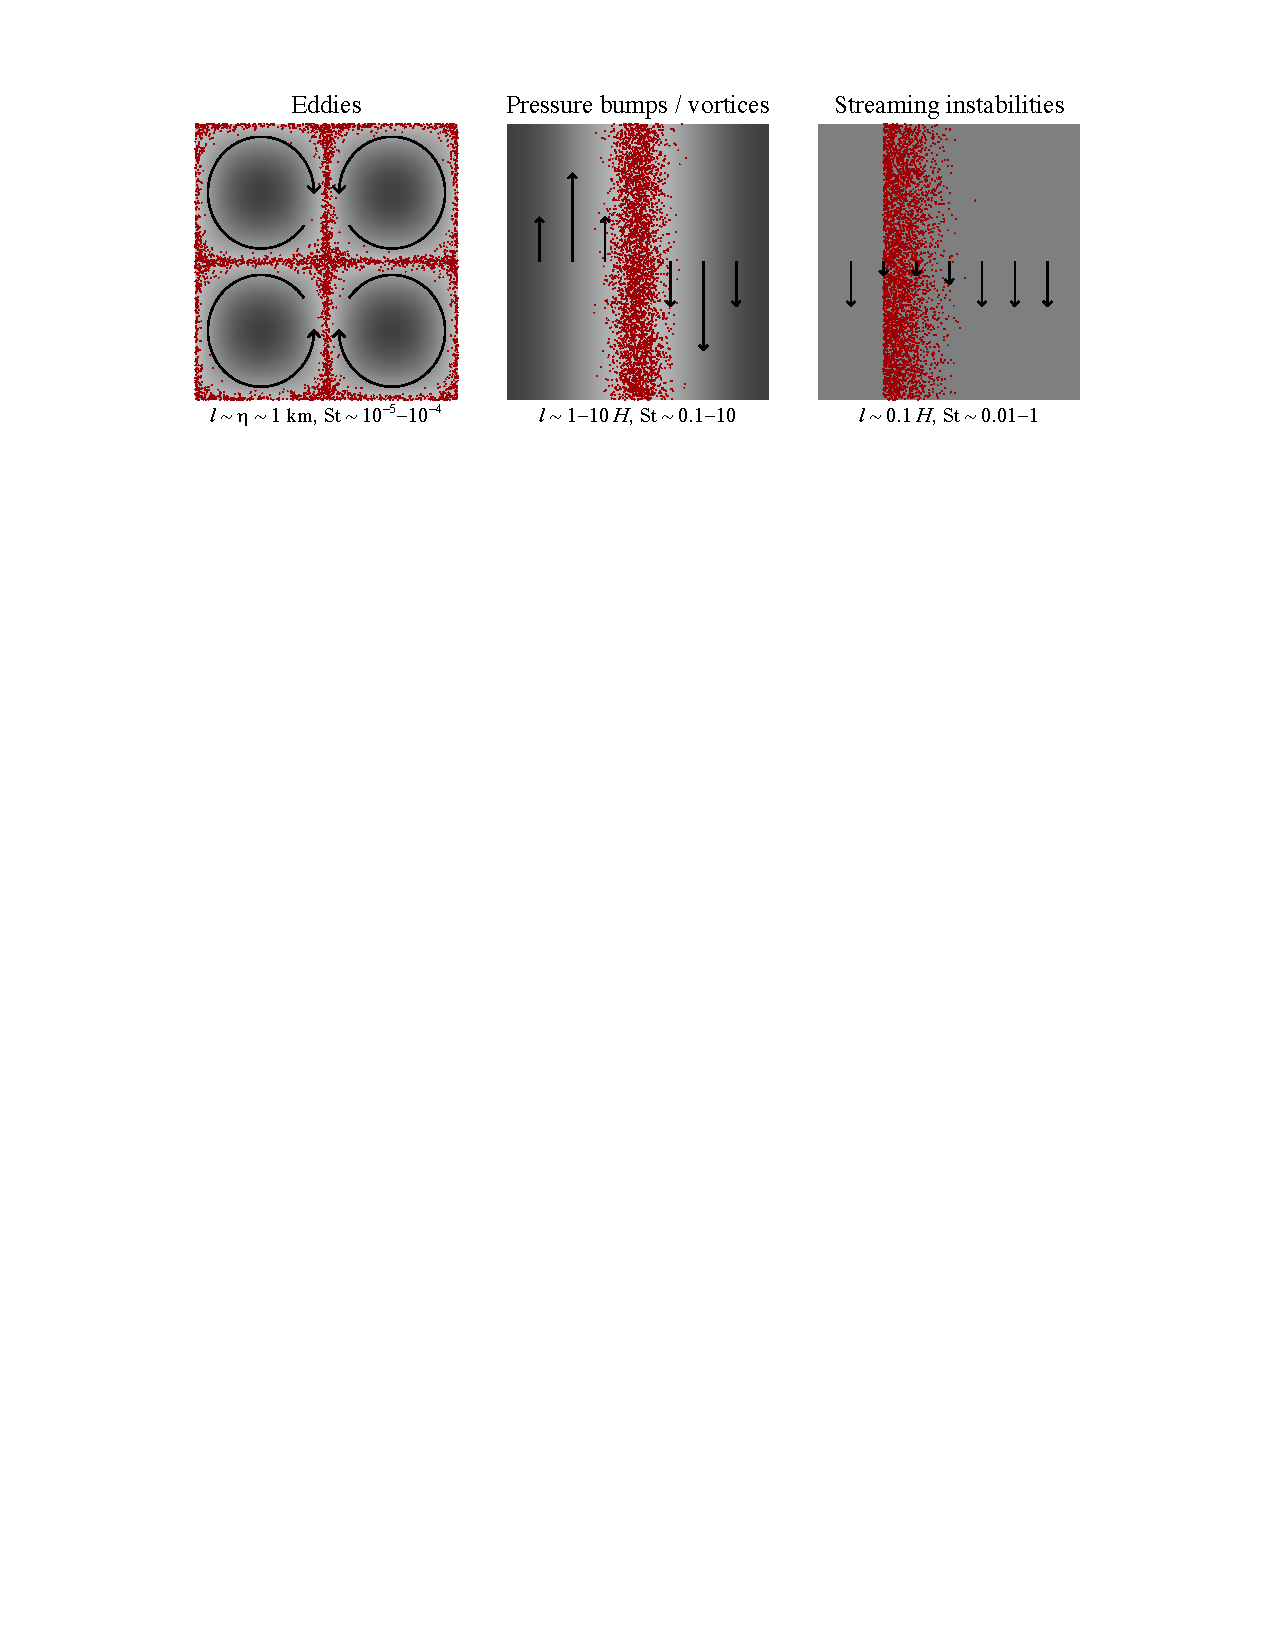
\includegraphics[width=\linewidth]{eddies_johansen14}
\caption[Schematic of particle concentration by eddies in a protoplanetary disk]{
\label{fig:eddies_johansen14a}
Schematic diagram of three mechanisms to concentrate particles in a protoplanetary disk, taken from \citet{johansen14a}. The left panel shows how small-scale turbulent eddies expel particles to their outskirts. The middle panel shows how zonal flows associated with large-scale pressure bumps concentrate particles. The right panel shows concentration by streaming instabilities. In each panel, black arrows show the velocity field, and the caption indicates the characteristic length scale of the structures shown, where $H$ is the disk scale height.
}
\end{figure}

The first mechanism we will examine is concentration of small particles by eddies in a disk (Figure \ref{fig:eddies_johansen14a}). Consider a rotating eddy in a disk. By an eddy here we mean a structure where the gas moves on circular trajectories in the frame co-rotating with the disk at angular velocity $\Omega$. Suppose that the gas at some distance $r$ from the center of an eddy is rotating at some speed $v_e$. In the rotating reference frame, there are two forces acting on the gas: pressure gradients and Coriolis forces. For the eddy to remain static, the sum of these two forces must produce an acceleration per unit mass equal to the centripetal acceleration associated with the circular motion of the eddy. Specifically, we must have
\begin{equation}
2\Omega v_e - \frac{1}{\rho} \frac{dP}{dr} = -\frac{v_e^2}{r},
\end{equation}
where the first term is the Coriolis force per unit mass, the second is the pressure force per unit mass, and the right hand side is the centripetal acceleration. For a slowly-rotating eddy, $v_e /r \ll \Omega$, we can ignore the right hand side, and simply approximate that the sum of the two terms on the left is zero. Thus for slow eddies, the eddy rotation speed is given by
\begin{equation}
v_e = \frac{1}{2\rho\Omega} \frac{dP}{dr}.
\end{equation}
We see that if the eddy is associated with a pressure maximum, $dP/dr < 0$, then $v_e < 0$ as well, indicating that rotation is clockwise; eddies associated with pressure minima, $dP/dr > 0$, produce counter-clockwise rotation.

Now let us consider the dynamics of a solid particle moving through the eddy. Returning to the inertial frame, if the eddy is rotating clockwise, $v_e < 0$, then the material that is further from the star is orbiting somewhat more slowly, while the material that is closer to the star is orbiting somewhat more rapidly. This means that the material farther from the star will have a smaller velocity difference with the sub-Keplerian solids, while the material that is closer to the star will have a somewhat larger velocity difference. The drag force is therefore smaller on the far side of the eddy, and larger on the near side. The net effect is that, as solids drift from large radii inward and encounter the eddy, their rate of drift slows down, and they tend to pile up at the location of the eddy. This is a potential mechanism to raise the local ratio of solids to gas, and thus to set off gravitational instability.

The final step in this argument is to have something that provides a pressure jump and thus can produce clockwise eddies. There are a number of possible mechanisms, including a build-up of gas at the edge of a dead zone where MRI shuts off, or simply the turbulence driven by the MRI itself. Whether this actually happens in practice is still an unsolved problem, but the mechanism is at least potentially viable.

Another possible mechanism to concentrate particles is known as the streaming instability. We will not derive this rigorously, but we can describe it qualitatively. Streaming instability operates as follows: suppose that, in some region of the disk, for whatever reason, the local density of solids relative to gas is slightly enhanced. Because we are in a mid-plane layer that is at least partly sedimented, the inertia of the solids is non-negligible. Thus while we have focused on the drag force exerted by the gas on the solids, the corresponding force on gas is not entirely negligible. This force tries to make the gas rotate faster, and thus closer to Keplerian. This in turn reduces the difference in gas and solid velocities.

Now consider the implications of this: where the solid to gas ratio is enhanced, the solids force the gas to rotate closer to their velocity, which in turn reduces the drag force and thus the inward drift speed. Thus if solid particles are drifting inward, when the encounter a region of enhanced solid density, they will slow down and linger in that region. This constitutes an instability, because the slowing down of the drift enhances the solid density even further, potentially leading to a runaway instead in the gas to solid ratio. If this mechanism is able to increase the ratio enough, gravitational instability will take over and produce planetesimals.




